\chapter*{Section 1} \label{section1}
\section{Problem Description}
For this work, we were given the task to create a dashboard 
that could simulate a real-time, real-world system for wildfire 
prevention. \par
In order to fulfil the above-mentioned objective, 
we were required to select one of two districts, 
namely Aveiro or Viseu. Our task was to analyse both districts, 
with a particular focus on the forest area in each. 
This area was considered crucial, since that it would be 
the location of the deployment of cameras and sensors, 
which would be used to collect data essential for preventing forest fires. 
To achieve
that goal, Silvanet Wildfire Sensors and Mesh Gateways are necessary to
survey and detect wildfires effectively. \par
In this particular instance, the decision was taken to select the Aveiro district. The district is situated in close proximity to our location, which constitutes one of the factors that led to our decision to select it. As illustrated in the district maps below, this district is characterised by a significant forest area. To be more precise, the total area of the Aveiro district is approximately 2808 km², with the forest area accounting for approximately 1400 km². \par
Furthermore, the district has 4,485 sensors and 446 gateways at the disposal of civil protection agencies. \par
\begin{figure}[H]
    \centering
    \begin{subfigure}[b]{0.5\textwidth}
        \centering 
        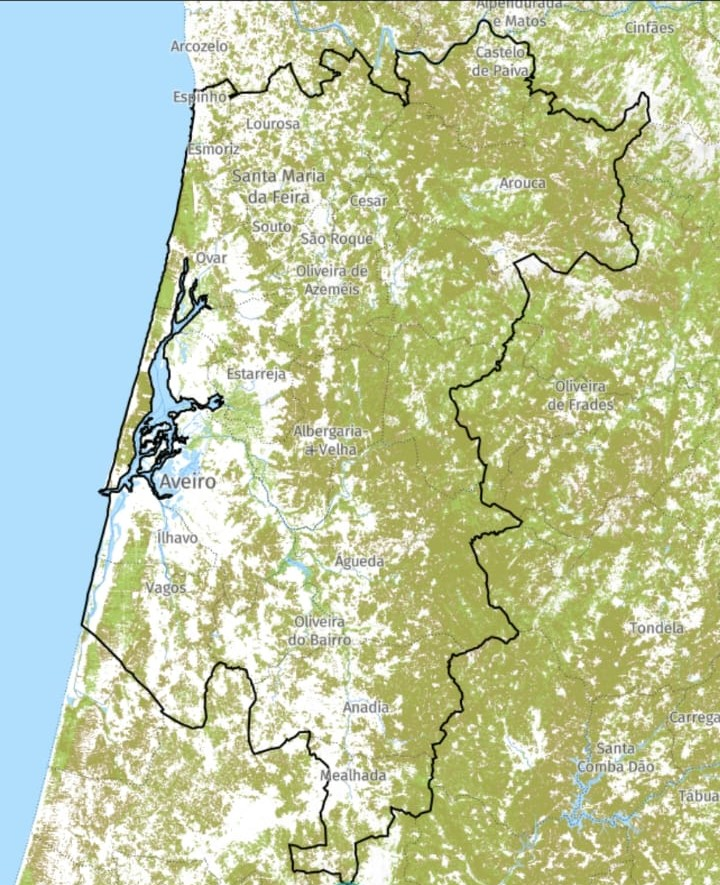
\includegraphics[width=0.8\textwidth]{Aveiro.jpg}
        \caption{Aveiro District Map}
    \end{subfigure}%
    \begin{subfigure}[b]{0.5\textwidth}
        \centering 
        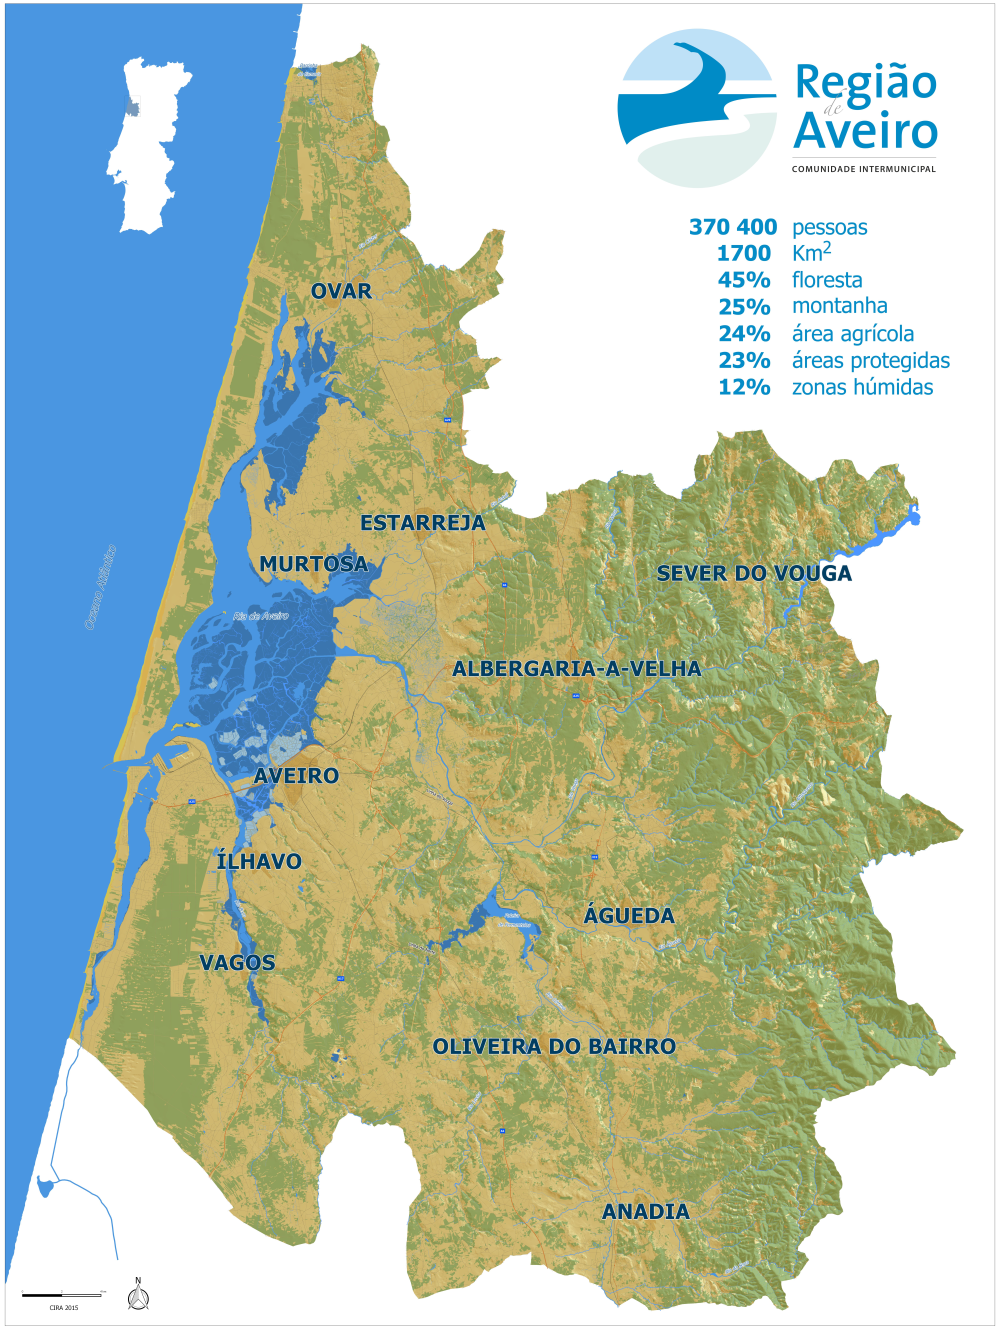
\includegraphics[width=0.8\textwidth]{mapahall_1_1250_2500.png}
        \caption{Aveiro Region Map}
    \end{subfigure}
    \caption{Aveiro Maps}
\end{figure}
\section{Biggest Challenges}
One of the biggest challenges we faced was keeping a complex system, with multiple functionalities, simple
and intuitive to use without the need for prior knowledge on this
specialized tech, such as the sensors and gateways. 
\section{Identification of Stakeholders}
In the context of this project, "stakeholders" can be defined as follows:
\begin{itemize}
    \item Dryad (Sensor Manufacturer)
    \item Firefighters
    \item SIRESP - Portuguese National Emergency 
    and Security Networks Operator 
    \item ANEPC - National Emergency and Civil Protection Authority
    \item City Council
    \item System Operators (from Civil Protection)
\end{itemize} \par 
All of these entities play a crucial role in the process of fire monitoring and firefighting. 
Civil Protection agencies and firefighters rely on this 
interface to facilitate effective emergency responses and 
ensure public safety. Sensor and camera manufacturers contribute 
valuable technology that is essential for accurate data capture, 
enabling timely and precise detection. Local authorities have 
a vested interest in protecting their local areas and resources, 
and benefit from a tool that enhances their preparedness and 
risk management strategies. Finally, system operators are integral 
to ensure smooth operations, maintenance, and real-time monitoring 
capabilities which, in turn, make it possible for all stakeholders 
to rely on accurate and up-to-date information. 
\section{Personas as Potential Users}
In order to come up with some of the sketches shown in Chapter \ref{section2},
we created two fictional personas, in this case, two 
fictional potential users of the system. In the end, we came up 
with the following:
 \\

\textbf{Persona 1:} \\
\begin{wrapfigure}{l}{0.25\textwidth}
    \begin{center}
    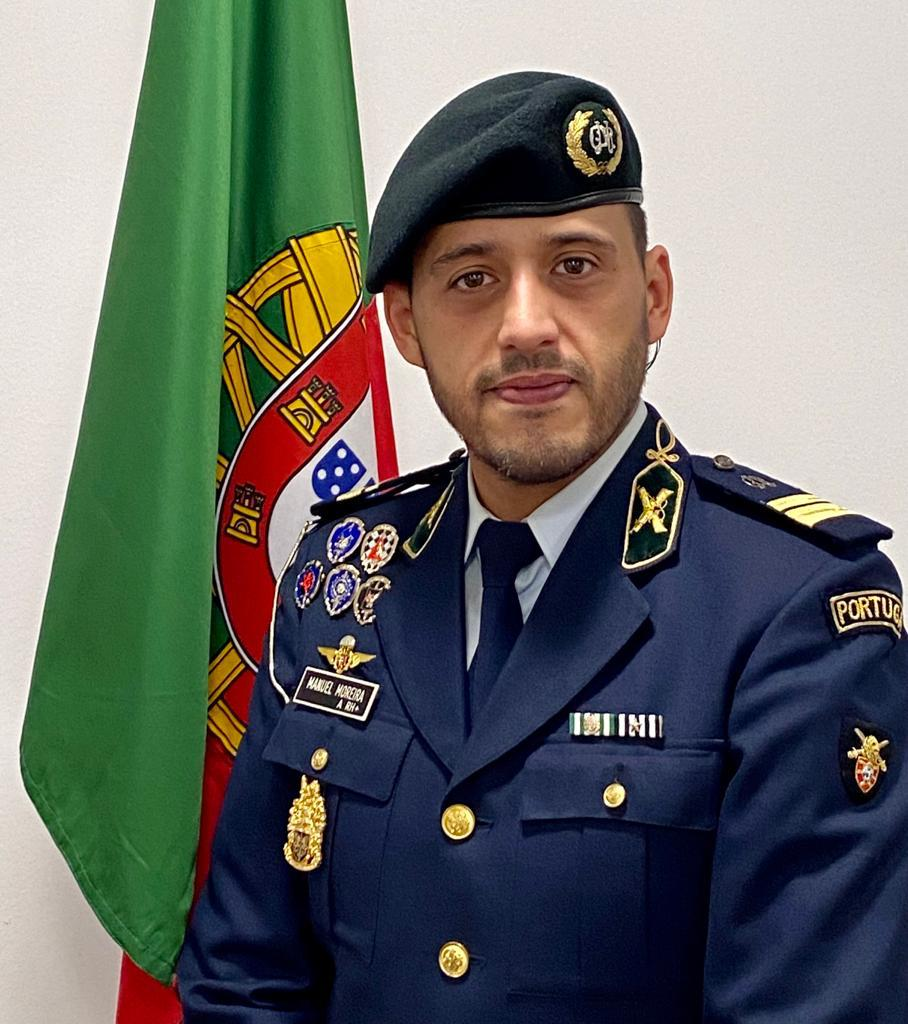
\includegraphics[width=0.25\textwidth]{personas/persona1.jpg}
    \end{center}
\end{wrapfigure}
\begin{itemize}
    \item Joaquim Soares (35 years old):
    \begin{itemize}
    \item Civil Protection agent;
    \item Lives with his wife and kids in Aveiro;
    \item Joined GNR and received police training at the age of 20;
    \item Worked as GNR in Aveiro's district during the wildfires of 
    Summer of 2024. 
    After this catastrophic experience, he volunteered to become a
    Civil Protection Agent in this new program to prevent and fight forest wildfires. \\
    \end{itemize}
\end{itemize} 

\textbf{Persona 2:} \\
\begin{wrapfigure}{l}{0.25\textwidth}
    \begin{center}
    
\includegraphics[width=0.25\textwidth]{personas/persona2.jpg}
    \end{center}
\end{wrapfigure}
\begin{itemize}
    \item João Rodrigues (24 years old):
    \begin{itemize}
    \item Has a degree in Management of
    Safety, Emergency, and Civil Protection;
    \item Lives with his parents and sister in Aveiro;
    \item Currently undertaking a post-graduation degree in Civil Protection,
    through online classes;
    \item Works as an operations assistant for Civil Protection; 
    \item Has ambitions to
    climb the ranks in ANEPC by gathering experience in various fields.
    \end{itemize}
\end{itemize}
